\documentclass[border=10pt]{standalone}
\usepackage{pgfplots}
\pgfplotsset{compat=1.18}
\begin{document}
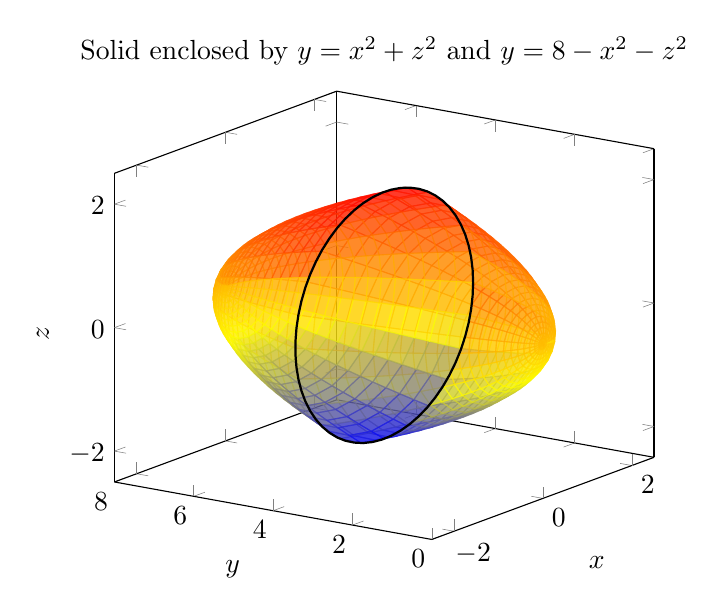
\begin{tikzpicture}
\begin{axis}[
    view={-55}{18},
    xlabel={$x$}, ylabel={$y$}, zlabel={$z$},
    xmin=-2.5, xmax=2.5, ymin=0, ymax=8, zmin=-2.5, zmax=2.5,
    domain=0:2, y domain=0:360,
    samples=25, samples y=25,
    colormap/hot,
    title={Solid enclosed by $y=x^2+z^2$ and $y=8-x^2-z^2$}
]
% Lower paraboloid y = x^2 + z^2 = r^2
\addplot3[surf, shader=flat, opacity=0.6]
    ({x*cos(y)}, {x^2}, {x*sin(y)});
% Upper paraboloid y = 8 - x^2 - z^2 = 8 - r^2
\addplot3[surf, shader=flat, opacity=0.6]
    ({x*cos(y)}, {8-x^2}, {x*sin(y)});
% Rim circle r = 2, y = 4
\addplot3[black, thick, domain=0:360, samples=60]
    ({2*cos(x)}, {4}, {2*sin(x)});
\end{axis}
\end{tikzpicture}
\end{document}